\documentclass[12pt]{article}
\usepackage{amsgen,amsmath,amstext,amsbsy,amsopn,amssymb}
%\usepackage[dvips]{graphicx,color}
\usepackage{graphicx,color,bm}
\usepackage{epsfig}
\usepackage{enumerate}
\usepackage{float}
\usepackage{multicol}
\usepackage{longtable}
\usepackage{verbatim}
\usepackage{hyperref}
\usepackage[utf8]{inputenc}
\usepackage[english]{babel}
\usepackage{commath}
\usepackage{tikz}
\usepackage{wrapfig,lipsum,booktabs}
%\setlength{\oddsidemargin}{0.1 in} \setlength{\evensidemargin}{-0.1
%in} \setlength{\topmargin}{-0.6 in} \setlength{\textwidth}{6.5 in}
%\setlength{\textheight}{8.5 in} \setlength{\headsep}{0.75 in}
%\setlength{\parindent}{0 in} \setlength{\parskip}{0.1 in}

\textwidth 6.3in \textheight 8.8in \topmargin -0.5truein
\oddsidemargin .15truein
\parskip .1in
\renewcommand{\baselinestretch}{1.00}  % double spaced
\renewcommand{\thesection}{\Roman{section}} 
\renewcommand{\thesubsection}{\thesection.\Roman{subsection}}
\newcommand*{\addheight}[2][.5ex]{%
	\raisebox{0pt}[\dimexpr\height+(#1)\relax]{#2}%
}
\usepackage{caption}

\begin{document}
	
\title{Homework 2, CSE 515}
\author{\bf Alexander Van Roijen}

\maketitle
	
\section{3.2}
\subsection{a}
For each graph there are three edges and thus 6 cases total, so we will show that no matter which edge from which graph we remove, we introduce an independency that was not implied originaly.
\\
\\
To clarify, we know that $P(x_1|x_2,x_3,x_4) = P(x_1|x_2) = P(x_1|x_3) = P(x_1|x_4)$, and that the same goes for any of our other random variables.
\\
\\
In our first graph, if we remove edge (3,4), we have $P(x_3|x_1,x_2,x_4) = P(x_3)$ which is certainly not true of $\mu$
\\
If we remove edge (1,4) we have $P(x_4|x_1) = P(x_4)$ which again is not true.
\\
Finally, if we remove edge (2,1) we have similar to removing edge (3,4) $P(x_2|x_1,x_3,x_4) = P(x_2)$ which is not true
\\
\\
In our second graph, removing edge (1,2) or (3,4) results in the same consequences as listed above in the first graph when removing the same edges. However, if we remove edge (3,1) we have $P(x_4|x_1) = P(x_4)$ which is again not true
\subsection{b}
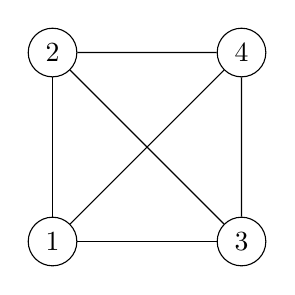
\begin{tikzpicture}
[scale=.8,auto=left,every node/.style={circle,draw=black}]
\node (n1) at (1,1) {1};
\node (n2) at (1,4)  {2};
\node (n3) at (4,1)  {3};
\node (n4) at (4,4) {4};

\foreach \from/\to in {n1/n2,n2/n3,n3/n4,n2/n4,n1/n3,n1/n4}
\draw (\from) -- (\to);
\end{tikzpicture}
\\\\
Our rule simply states to remove an edge i,j if it satisfies $x_i \perp x_j | x_{rest}$ which we know is true in all cases. thus we get the disconnected graph 
\\
\\
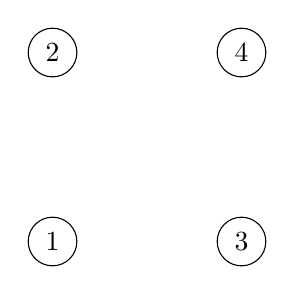
\begin{tikzpicture}
[scale=.8,auto=left,every node/.style={circle,draw=black}]
\node (n1) at (1,1) {1};
\node (n2) at (1,4)  {2};
\node (n3) at (4,1)  {3};
\node (n4) at (4,4) {4};
\end{tikzpicture}
\\
\\
This clearly is no longer a valid imap

\subsection{c}

Using the same graph above, which shows a completely disconnected graph, we have satisfied the pairwise markov property, as any two nodes, conditioned on the remaining two, is independent of each other. However, the local markov property is not satisfied as there are no neighbors $\partial i$ to condition on, and it is certainly not true that $X_i \perp X_j | \emptyset$ $\square$.
\subsection{d}
We know that given two disjoint subsets $A,C$ separated by another subset $B$, with the global markov property  we have $X_A\perp X_C | X_B$. It is simple to see that this implies our local markov property. We know that since A and C are separated by B, there are no edges between any edge $(a,c)$ $a \in A, c\in C$ which further means $\forall (a,c)$ $a \in A, c\in C$ $x_a \perp x_c | X_B$. This means one of two things, either $\forall e \in E(A)$ $e\in (a,b)$ or $(a_1,a_2)$ where $a_1,a_2\in A$ which means in the most general case $x_a \perp x_c | E(a)$ where $E(a)$ represents all edges containing node $a$ which is equivalently $x_a\perp x_c | \partial(a)$. However we can still go further by relabeling what our $B$ is. If we consider $B=\partial a$, we get from the global markov property that $x_a\perp X_C | X_B$, where our C now contains all nodes $c$ where B seperates C which is exactly $V - \{a,\partial{a}\} \rightarrow x_a - x_{\partial a} - X_{V - \{a,\partial{a}\}}$
\subsection{e}
This is another rather intuitive result, and is because separation is monotonic in our markov network (meaning super sets of Z provide the same conditional independencies as Z). From the local markov property, we know that given the neighbors, or all adjacent nodes and the edges between them and some other node $X_i$ we are independent of the remaining nodes $\chi - {X_i, X_{\partial i}}$. This directly implies the pairwise property as the set of $\chi - {X_i, X_{\partial i}} \subset \chi - {X_i,X_j}$. Thus, since we know that both our edges and respective variables that imply conditional independence from the local markov property are subsets of the pairwise, we are given the results of the pairwise property as $X\perp Y | Z \rightarrow X\perp Y | Z,A$ in a markov network where $A$ is some random variable in $\chi - {X,Y,Z}$  
\section{3.3}
\begin{comment}
	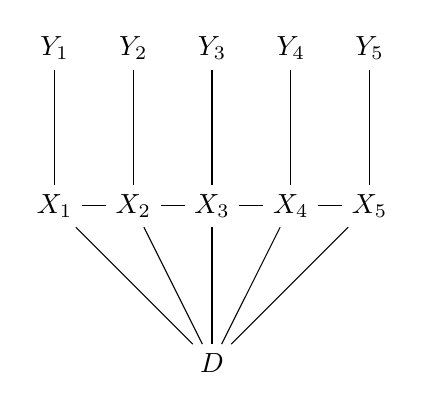
\begin{tikzpicture}
	
	[scale=.8,auto=left,every node/.style={circle,draw=black}]
	\node (x1) at (1,3) {$X_1$};
	\node (x2) at (2,3) {$X_2$};
	\node (x3) at (3,3) {$X_3$};
	\node (x4) at (4,3) {$X_4$};
	\node (x5) at (5,3) {$X_5$};
	\node (y1) at (1,5) {$Y_1$};
	\node (y2) at (2,5) {$Y_2$};
	\node (y3) at (3,5) {$Y_3$};
	\node (y4) at (4,5) {$Y_4$};
	\node (y5) at (5,5) {$Y_5$};
	\node (d) at (3,1) {$D$};
	
	\foreach \from/\to in {x1/x2,x2/x3,x3/x4,x4/x5,x1/y1,x2/y2,x3/y3,x4/y4,x5/y5,x1/d,x2/d,x3/d,x4/d,x5/d}
	\draw (\from) -- (\to);
	\end{tikzpicture}
\end{comment}


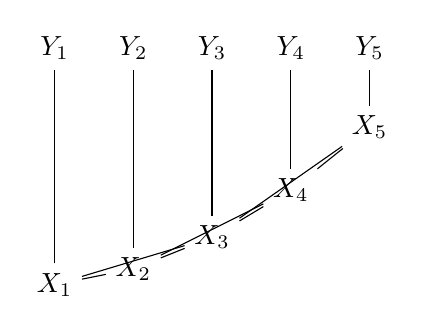
\begin{tikzpicture}

[scale=.8,auto=left,every node/.style={circle,draw=black}]
\node (x1) at (1,3) {$X_1$};
\node (x2) at (2,3.2) {$X_2$};
\node (x3) at (3,3.6) {$X_3$};
\node (x4) at (4,4.2) {$X_4$};
\node (x5) at (5,5) {$X_5$};
\node (y1) at (1,6) {$Y_1$};
\node (y2) at (2,6) {$Y_2$};
\node (y3) at (3,6) {$Y_3$};
\node (y4) at (4,6) {$Y_4$};
\node (y5) at (5,6) {$Y_5$};

\foreach \from/\to in {x1/x2,x2/x3,x3/x4,x4/x5,x1/y1,x2/y2,x3/y3,x4/y4,x5/y5,x1/x3,x2/x4,x3/x5}
\draw (\from) -- (\to);
\end{tikzpicture}
\\
I apologize for the picture, i wasnt sure how to create curved lines here in latex, but basically I am demonstrating that for $X_i$ where $i > 2$ depends on $x_{i-1},x_{i-2}$
\\\\
We know that the duration is at most two, so in this case, having knowledge of the previous two states tells us as much as we can, regardless of if d = 1 or d = 2. In the case d = 1, we see the transition in the previous two states, if not and d = 2, we know we will be transitioning now. You can imagine it as $P(X_i|X_{i-1},X_{i-2}) = I(x_{i-1} = x_{i-2}) P_T(X_i|x_{i-1}) + I(x_{i-1} != x_{i-2})P_D(1)P_T(X_i|x_{i-1}) + I(x_{i-1} != x_{i-2})P_D(2)$. Clearly, removing any edge between y and X would be improper as Y and associated X are exactly dependent on each other, and removing any edge between the $X_i$ established would add improper additional independencies not expressed by our factorization.
\subsection{b}
$\phi(x_i,x_{i+1},t_i) = P_T(x_{i+1}|x_{i})P_D(t_i)$
\\
$\xi(x_i,t_i)= \Sigma_{i=t+1}P_D(d= i)$
\\
$\tilde{P}(Y_i|X_i,T_i) = P_{Yi|Xi}(Y_i|X_i)$
\subsection{c}
In general, we are trying to solve $P(X_N) = \Sigma_{X_{N-1},..,X_1}P(X_N|X_{N-1},..,X_1)$ which, in the absolute worst case, take $ \chi^{|V|} = (KM)^N$ as we know the alphabet is of size $KM$. However, we know that this can be reduced to $N(KM)^2$ since we know $v_{i+1 \rightarrow i+2} (X_{i+1}) = v_{i \rightarrow i+1} (X_{i}) \phi(x_i,t_i,x_{i+1},t_{i+1})$. However, this can be reduced. For any node in general, excluding edge cases, we have two cases.\\
\\
Case 1: $X_i = X_{i+1} $ This means that we are concerned only with $v_{i+1 \rightarrow i+2} (X_{i+1}) \propto \xi(x_i,t_i)= \Sigma_{i=t+1}P_D(d= i)$. Which would take $kM$ time, as we have k possible situations where $X_i = X_{i+1} $
\\
\\
Case 2: $X_i \ne X_{i+1} $. This means that we are concerned only with $v_{i+1 \rightarrow i+2} (X_{i+1}) \propto \phi(x_i,x_{i+1},t_i) = P_T(x_{i+1}|x_{i})P_D(t_i)$. However, $P_D(t_i)$ is a constant, and takes constant time to calculate. So we have that this takes $O(k^2)$ as we have $k^2$ possible combinations of $X_i \ne X_{i+1}$. Technically, its $k(k-1)$, but this is roughly $k^2$.
\\
\\
Combining this, we know that for each of our $N$ nodes, we have $O(k^2 +kM)$ calculations, for each of our $v_{i+1 \rightarrow i+2} (X_{i+1})$. Thus our total run time for the sum product algorithm would be $O(N(k^2+kM))$
\section{4.1}
\subsection{a}
We will prove this via induction. 
\\
The base case is simple, as we have for $t=0$
$v^{\prime \, t}_{i\rightarrow j}(x_i) =v^{\, t+1}_{i\rightarrow j}(x_i) = v^{\prime \, 0}_{i\rightarrow j}(x_i) =v^{\, 1}_{i\rightarrow j}(x_i) $. This comes from the initialization.
\\
Now we assume for $t$ we have $v^{\prime \, t}_{i\rightarrow j}(x_i) =v^{\, t+1}_{i\rightarrow j}(x_i)$. And we need to show $v^{\prime \, t+1}_{i\rightarrow j}(x_i) =v^{\, t+2}_{i\rightarrow j}(x_i)$.
\begin{gather}
	v^{\prime \, t+1}_{i\rightarrow j}(X_i) = \Pi_{k\in \partial i - j} \Sigma_{x_k} \psi^\prime(x_k,x_i)v^{\prime \, t}_{k\rightarrow i}(x_k) \text{by definition}\\
	= \Pi_{k\in \partial i - j} \Sigma_{x_k} \psi(x_k,x_i)v^{\prime \, t}_{k\rightarrow i}(x_k) \text{given}\\
	= \Pi_{k\in \partial i - j} \Sigma_{x_k} \psi(x_k,x_i)v^{t+1}_{k\rightarrow i}(x_k) \text{ induction hypothesis}\\
	= v^{\, t+2}_{i\rightarrow j}(x_i) \text{ by definition} \square
\end{gather}
\subsection{b}
The diameter of a tree is the longest path between any two nodes or vertexes. Say we have two nodes $V_i$ and $V_j$ such that the distances between $V_i$,$V_j$ is maximal, which is defined as the number of edges between themselves, with a distance we call $D$. We know for one that if there was any edge and corresponding node $V_x$ that was associated with either $V_i$ or $V_j$, it must be in the path between $V_i$ or $V_j$. Otherwise, if it were, that would mean there is a longer path between $V_x$ and either $V_i$ or $V_j$ with length $D+1$, which would go against our assumption that we have found the path of the maximal length. With this in mind we know that by removing the leaves from our $T$ we have inherently reduced the longest path from $D$ to at least $D-1$. This is exactly because we know the maximal path is between leaves, and by removing them and creating new ones that are along the path of our previous diameter means it must be shorter. $\square$
\subsection{c}
Fortunately, the base case has already been justified, so now we need to show that given we know that a tree with diameter $d \le D-1$ converges on the sum product algorithm in at most $D-2$ time steps, that when we add the leaves back in, it will converge in one more time step, or $D-1$ time steps.
\\
We have that $v^{\prime \, t}_{i\rightarrow j}(x_i) =v^{\, t+1}_{i\rightarrow j}(x_i)$ which means $v^{\prime \, d-2}_{i\rightarrow j}(x_i) =v^{\, d-1}_{i\rightarrow j}(x_i)$. Which actually proves our convergence, as our $v^{\, d-1}_{i\rightarrow j}(x_i)$ is the message for our tree with the leaf nodes re-attached. Thus, since our $v^{\prime \, d-2}_{i\rightarrow j}(x_i)$ has converged in the $D-2$ steps, and we have shown the messages are equivalent for our original tree in $D-1$ time, which has the leaf nodes re-attached, it must have also reached convergence, in simply one more time step! $\square$
\section{4.2}
\subsection{a}
we have that $\phi(x_i,x_j) = e^{\theta_{ij}x_ix_j}e^{\frac{\theta_{i}x_i}{|E_{\partial i}|} }$ \\
This comes directly from our given join distribution function, as we can break it apart into this multiplication of compatibility functions. The reason for $|E_{\partial i}|$ is we need a normalizing term such that we get our original joint distribution back when we multiply them all together.
\\
\\
Plugging this into the general format of the message passing algorithm we get $v_{x_{i}\rightarrow x_{j}}(x_i) = \prod_{\partial i - j}^{x_k}\Sigma_{x_k}v_{x_k \rightarrow x_i}(x_k)e^{\theta_{ik}x_ix_k}e^{\frac{\theta_{i}x_i}{|E_{\partial i}|} }$
\\
This means $\frac{1}{2}\log(\frac{v_{x_{i}\rightarrow x_{j}}(+1)}{v_{x_{i}\rightarrow x_{j}}(-1)}) = \frac{1}{2}\log(\frac{\prod_{\partial i - j}^{x_k}\Sigma_{x_k}v_{x_k \rightarrow x_i}(x_k)e^{\theta_{ik}x_k}e^{\frac{\theta_{i}}{|E_{\partial i}|} }}
{\prod_{\partial i - j}^{x_k}\Sigma_{x_k}v_{x_k \rightarrow x_i}(x_k)e^{-\theta_{ik}x_k}e^{\frac{-\theta_{i}}{|E_{\partial i}|} }})$
\\
\\
This can be expanded to 
$\frac{1}{2}\log(\frac{\prod_{\partial i - j}^{x_k}
	(v_{x_k \rightarrow x_i}(1)e^{\theta_{ik}}e^{\frac{\theta_{i}}{|E_{\partial i}|} }
	+
	v_{x_k \rightarrow x_i}(-1)e^{-\theta_{ik}}e^{\frac{\theta_{i}}{|E_{\partial i}|} }	
	)}{\prod_{\partial i - j}^{x_k}(
	v_{x_k \rightarrow x_i}(1)e^{-\theta_{ik}}e^{\frac{-\theta_{i}}{|E_{\partial i}|} }
	+ 
	v_{x_k \rightarrow x_i}(-1)e^{\theta_{ik}}e^{\frac{\theta_{i}}{|E_{\partial i}|} })
})$
\\
\\
Now something tells me we can simplify this futher into some some of tans and arctans, but I am having a hard time figuring out how to do that. So for now this is what that log ratio would look like.
\subsection{b}
done
\subsection{c}
\begin{figure}[H]
	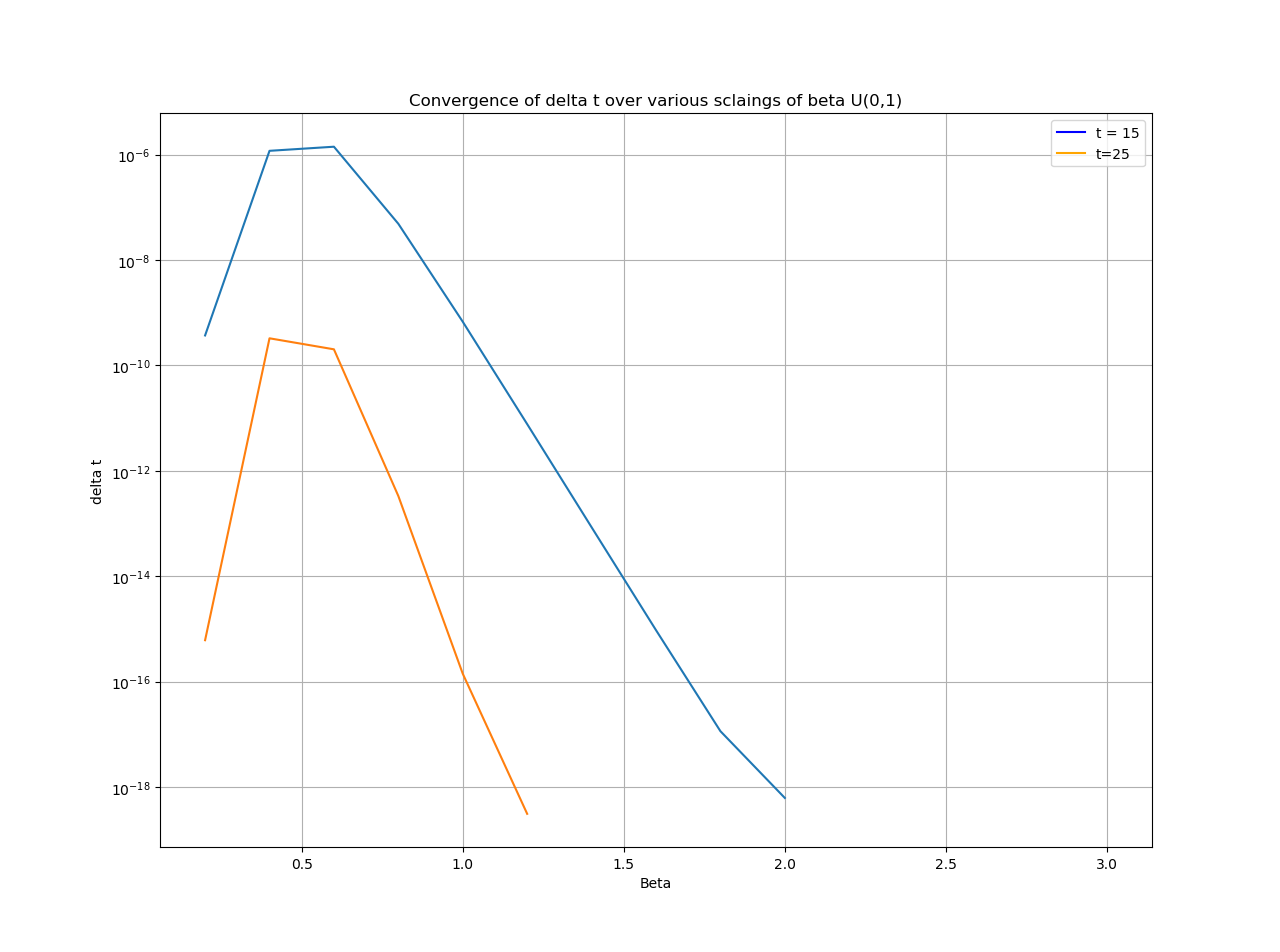
\includegraphics[width=0.8\textwidth]{q4_2_narrow.png}
	\caption{concavity of convergence of theta U(0,1)}
\end{figure}

We can see that with increasing iterations we see large to small differences in convergence based on the scale of our beta. There is an concave down relationship where certain values of scaling beta cause larger differences per iteration at our terminal time steps, in this case, this value is a $\beta = [0.4,0.6]$. However, on the other sides, the difference between messages at the terminal time step reduce greatly. This is likely due to the initialization of the thetas in that range of $\beta$
\subsection{d}
\begin{figure}[H]
	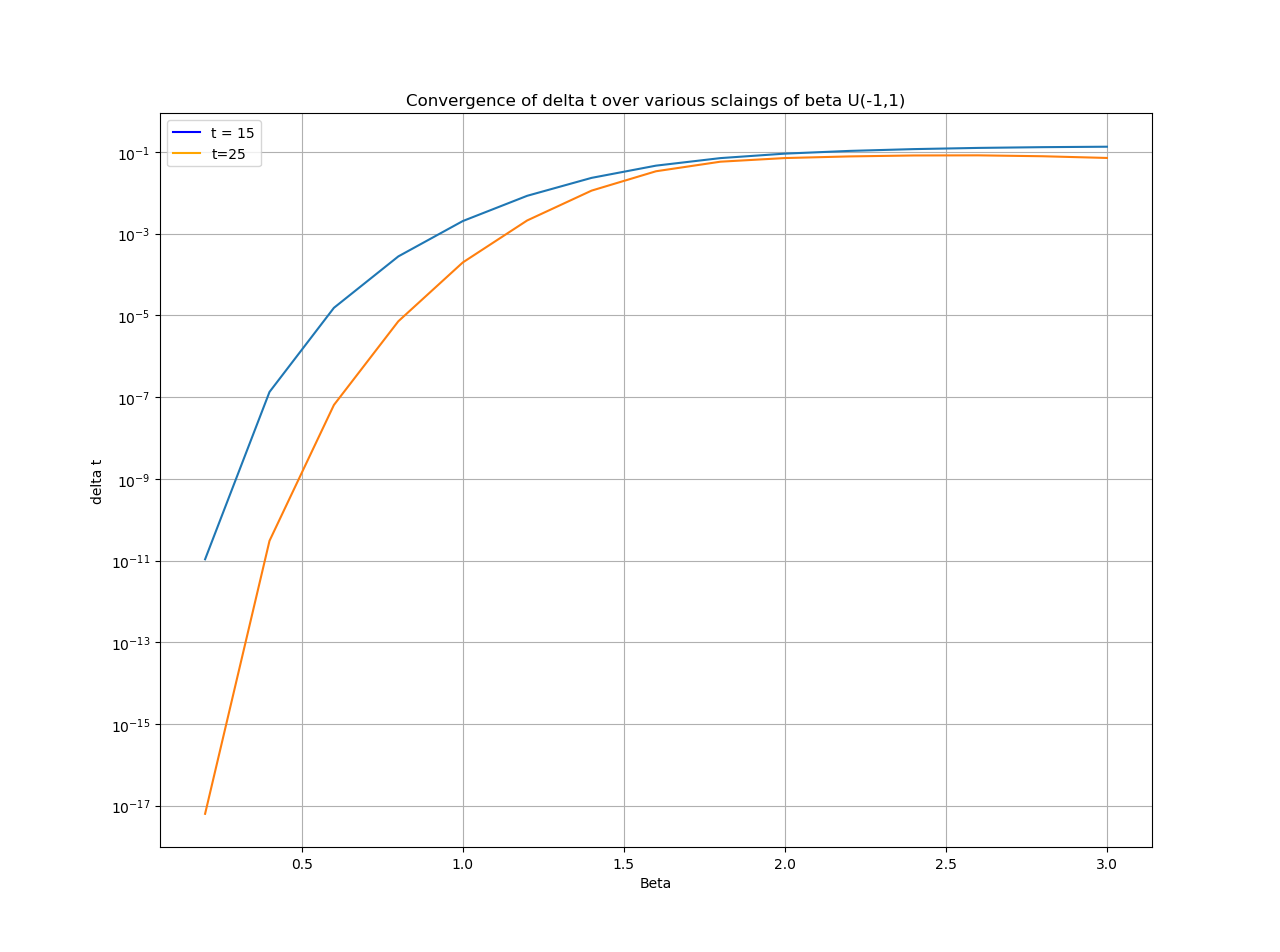
\includegraphics[width=0.7\textwidth]{q4_2_large.png}
	\caption{concavity of convergence of theta U(-1,1)}
\end{figure}
Unlike in our previous graph, there is no nice concave down relationship, instead it appears to plateau and increase in difference with increasing values of $\beta$. My intuition tells me that by allowing our initialization of $\theta$ to be negative cause greater divergence between messages in both orders of time steps to a point of no convergence. This is most likely due to the $e^{\theta_{ij}x_ix_j}$. If that theta is negative, the ability of the energies to evaluate to the proper sign amongst their neighbors becomes a greater challenge
\section{4.3}
\subsection{a}
\begin{figure}[H]
	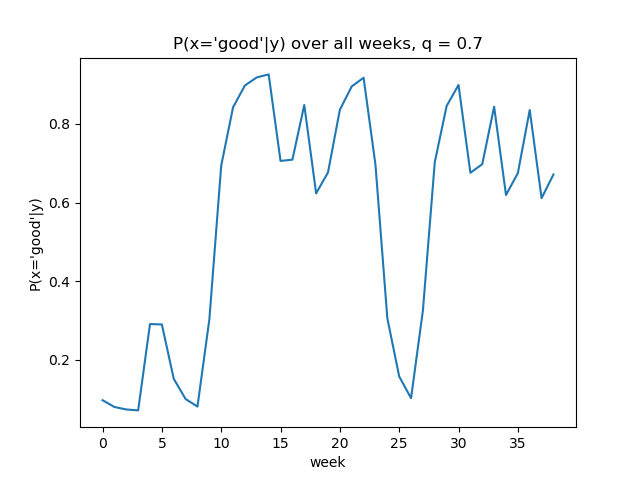
\includegraphics[width=0.7\textwidth]{q_0_7.png}
	\caption{Probability over the weeks with $q=0.7$}
\end{figure}
Since its hard to grab from the graph $P(x_{t=39}="good"|y) = 0.67$
\subsection{b}
\begin{figure}[H]
	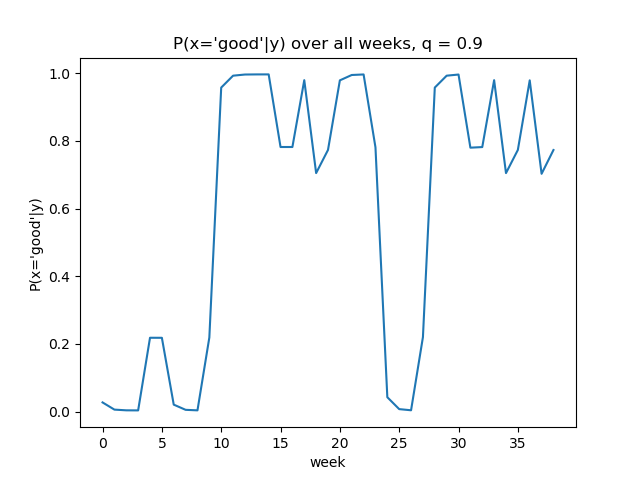
\includegraphics[width=0.7\textwidth]{q_0_9.png}
	\caption{Probability over the weeks with $q=0.9$}
\end{figure}
$P(x_{t=39}="good"|y) = 0.77$. Comparing these two, we can see that with a higher q, which represents a greater confidence in the market being in a good or bad state given the rise or fall of that given week, we get an overall greater confidence in the last state being in the good state given our series of observations

\begin{section}{Appendix}
	This code used to generate plots and more will be posted on github soon @ user: "bogyshi" https://github.com/bogyshi! stay posted!
	\\
	\\
	Question 4.3 code
	\begin{verbatim}
		#!/usr/bin/env python
		# coding: utf-8
		
		import numpy as np
		import matplotlib.pyplot as plt
		
		
		stockData = np.genfromtxt('sp500.csv', delimiter=',')
		
		print(stockData)
		print(len(stockData))
		q=0.9
		p_up_good = q
		p_up_bad = 1 - p_up_good
		upPs = np.array([p_up_good,p_up_bad])
		p_down_good=1-q
		p_down_bad = 1-p_down_good
		downPs = np.array([p_down_good,p_down_bad])
		initPs2 = np.array([[p_up_good,p_up_bad],[p_down_good,p_down_bad]])
		updownMatrix = np.array([[0.8,0.2],[0.2,0.8]]) # being in the good state is top row, bad state is bottom, 1st col represents good prob, second represent bas prob
		
		pStay = 0.8
		pChange = 0.2
		
		def sumProdRecursive(data,index):
		ps = np.array([0,0])
		if(index == len(data)):
		return np.array([0.2,0.8])
		else:
		message = sumProd(data,index-1)
		
		
		
		def sumProdIter(data):
		totalProbOfEvents=1
		lenData = len(data)
		i = 0
		measurements = []
		initPs = np.array([0.2,0.8])
		message = initPs
		while(i<lenData):
		pGood = message[0]
		pBad = message[1]
		updown = data[i]
		if(updown == 1):
		diagMatrix = np.diag(initPs2[:,0]) # up on top, down on bottom, good state 0th col, bad state 1th col
		top = p_up_good*pGood
		bottom = p_up_good*pGood + p_up_bad*pBad
		#message[0] = (pGood*pStay*p_up_good + pBad*pChange*p_up_good)
		#message[1] = (pBad*pStay*p_up_bad + pGood*pChange*p_up_bad)
		else:
		diagMatrix = np.diag(initPs2[:,1])
		top = p_down_good*pGood
		bottom = p_down_good*pGood + p_down_bad*pBad
		#message[0] = (pGood*pStay*p_down_good + pBad*pChange*p_down_good)
		#message[1] = (pBad*pStay*p_down_bad + pGood*pChange*p_down_bad)
		ptop = top/bottom
		totalProbOfEvents = totalProbOfEvents*np.sum(message.dot(updownMatrix).dot(diagMatrix))
		message = message.dot(updownMatrix).dot(diagMatrix)/np.sum(message.dot(updownMatrix).dot(diagMatrix))
		print(message)
		print(ptop)
		
		#message[0] = (pGood*pStay + pBad*pChange)*ptop
		#message[1] = (pBad*pStay + pGood*pChange)*ptop
		measurements.append(ptop)
		i+=1
		return measurements,totalProbOfEvents
		res,totalProbOfEvents2= (sumProdIter(stockData))
		print(totalProbOfEvents2)
		
		plt.plot(res)
		plt.title("P(x='good'|y) over all weeks, q = " + str(q))
		plt.xlabel("week")
		plt.ylabel("P(x='good'|y)")
		plt.show()
		\end{verbatim}
\end{section}



\end{document}